

    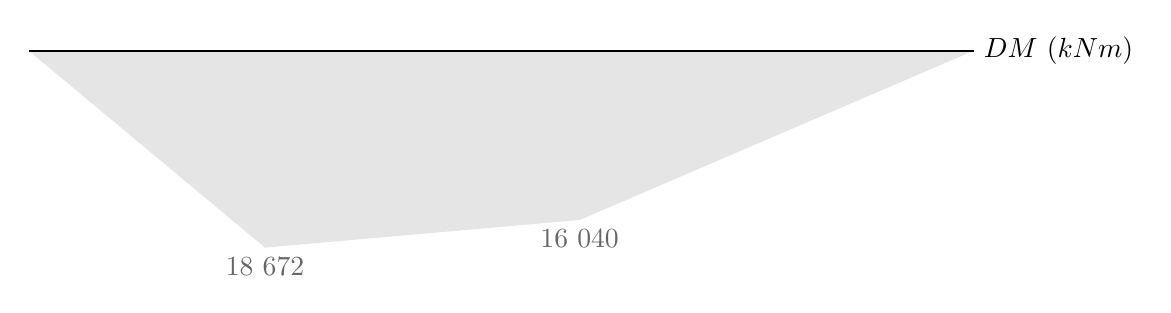
\begin{tikzpicture}
        % 1. VARIÁVEIS
        \def\L{12}   % Comprimento total da viga (eixo x)
        \def\V{2.5}  % Altura máxima do gráfico (representando os 40 kNm)

        % ==========================================
        % 2. EIXO DE REFERÊNCIA
        % ==========================================
        \draw[thick, gray] (0, 0) -- (\L, 0) node[right, text=black] {$DM \ (kNm)$};

        % ==========================================
        % 3. PREENCHIMENTO E CONTORNO PROPORCIONAL
        % ==========================================
        % Altura Y = 100% de \V (referente aos 40 kNm)
        % Posição X = 4m é um terço de L (\L/3) e 8m são dois terços (2*\L/3)
        \fill[gray!20] (0,0) -- (0.25*\L, -\V) -- (0.583*\L, -0.86*\V) -- (\L, 0) -- cycle;
        
        % Reforça a linha do eixo central em preto
        \draw[thick, black] (0,0) -- (\L,0);

        % ==========================================
        % 4. RÓTULOS, VALORES E GUIAS
        % ==========================================
        % Valores do momento máximo posicionados na cota -\V
        \node[below, gray!80!black] at (0.25*\L, -\V) {$18 \ 672$};
        \node[below, gray!80!black] at (0.583*\L, -0.86*\V) {$16\ 040$};

    \end{tikzpicture}